\section{4. Protein structure prediction}

\begin{framed}
\textbf{Learning outcomes}\\
\begin{itemize}
\item 1
\item 2
\item 3
\end{itemize}
\end{framed}

\subsection{Predicting protein structures: the sequence-structure-function paradigm}

A lot of sequences have become available.
However, for most, we do not yet know what type of proteins they represent, and what functionality they have.

Proteins are essential for life on earth.
They have many kinds of functions in organisms such as supporting its structure (e.g., keratin in our skin), performing enzymatic reactions (e.g., Ribulose-1,5-bisphosphate carboxylase-oxygenase, a.k.a. Rubisco, in plants), or receptors for transduction of signals that mediate cell-to-cell communication.
As discussed in chapter~1, only a relatively small amount of amino acid building blocks forms the basis of a structurally very diverse protein repertoire.
Hence, to understand the function of proteins, knowing their structures is key. In chapter~1 you have also learned that proteins are created as a long chain of amino acids held together by peptide bonds, i.e., a polypeptide chain (the primary structure), that folds into a three-dimensional (tertiary) structure, based on various types of interactions between amino acid side groups.
Usually, during this folding process, shorter stretches of local 2D (secondary) structures form first, held together by hydrogen bonds.
Interestingly, whereas the amino acid sequence of proteins may differ, their folding may still result in comparable 3D structures of the polypeptide chain -- with comparable or even similar functionality (see Figure~\ref{myoglobin}).
Several folded polypeptide chains can form the final quaternary complex that is functional within the cell.
Thus, the protein folding process is important, as it determines the 3D structure of polypeptide chains, and misfolding can lead to misfunctioning of the protein, for example by non-specific binding to other proteins, causing a disease in humans, or a less-performing mutant in plants.

\begin{figure}[!htbp]
\centering
\includegraphics[width=0.8\linewidth]{files/myoglobin-3a26c60b663bcd193d194d3391d896b0.png}
\caption[]{Protein structures of human myoglobin (top left), African elephant myoglobin (top right, 80\% sequence identity to human structure analogue), blackfin tuna myoglobin (bottom right, 45\% sequence identity to human analogue), and pigeon myoglobin (bottom left, 25\% sequence identity to human analogue).
Myoglobin can be found in muscles and its main function is to supply oxygen to muscle cells.
The protein structures in this figure illustrate how structure can be largely the same even for sequences that are quite different.
Credits: \cite{blopig_2021}.}
\label{myoglobin}
\end{figure}

While current experimental methods can generate many sequences of hypothetical proteins present in organisms, it is still hard and expensive to determine the corresponding 3D protein structures experimentally.
The main traditional experimental analytical techniques used are nuclear magnetic resonance (NMR) spectroscopy and X-ray crystallography.
The former yields useful but often noisy measurements with usually multiple structural conformations; whereas the latter is more accurate, but easily costs 120,000 euros. Furthermore, it can take a year or even longer to fully elucidate the protein 3D structure from the data, and some structures cannot be measured at all, for example due to crystallization problems.
Fortunately, fueled by recent technical advances, biological sequence data has become widely available, mostly in the form of genomic sequences.
By translating these DNA sequences into possible amino acid sequences using the codon language you have learned about in chapter~1, amino acid sequences can be inferred in which theoretical proteins can be predicted.
However, the sheer number of biological sequences make manual analysis of such predicted protein sequences too daunting. Thus, alternative methods to derive 3D protein structures are needed to interpret the large amount of biological sequence data that has become available in the recent decades.
Consequently, predicting protein structures based on protein sequence information has been a topic of high interest and relevance to biochemists~and scientists in general for many decades.

The sequence-structure-function paradigm states that, \textit{in principle}, all information to predict the folding of a protein, and thus its 3D structure and ultimately its function, is stored in its primary sequence.
In practice, however, predicting structure from its sequence turned out to be a very complex and challenging task.
One of the reasons for this complexity is due to the both short- and long-range interactions between protein local structure elements, i.e., interactions between secondary structure (2D) elements such as sheets and helices typically form anchor points upon which the tertiary (3D) structure is based.
This chapter first describes 2D structure assignment and prediction, after which foundational 3D structure prediction approaches are discussed, including the main challenges and the three zones of tertiary structure prediction.
It ends with the most recent approaches to predict and compare tertiary structures: AlphaFold and Foldseek.


\bigskip
\centerline{\rule{13cm}{0.4pt}}
\bigskip

\subsection{Secondary protein structure prediction}

Proteins consist of several locally defined secondary structure elements of which alpha helices ($\alpha$-helices) and beta strands/sheets ($\beta$-strands/sheets) are the most commonly occurring ones.
Please note here that a $\beta$-strand refers to one side of the $\beta$-sheet, where two strands come together to form the sheet structure.
In this section, we will cover how to assign these two secondary structure elements using 3D protein structures, and how to predict these secondary structure elements based on sequence data.
Furthermore, we will cover the prediction of two biologically relevant ``special cases'' of secondary structure elements: transmembrane sections and signaling peptides.


\bigskip
\centerline{\rule{13cm}{0.4pt}}
\bigskip

\subsubsection{Secondary structure assignment}\label{chapter4_secondary_structure_assignment}

If we consider the 3D structure of folded protein chains, we typically observe that the more ordered parts of their structures usually contain more $\alpha$-helices and $\beta$-strand stretches than the more randomly organized parts.
As these elements fold locally, they can initiate folding of more complex tertiary folding patterns. Indeed, the presence/absence of $\alpha$-helices and $\beta$-sheets and their specific conformation helps to categorize proteins.
As a result, databases exist that categorize proteins according to specific fold types, in a structured, hierarchical way.
Therefore, the assignment of amino acid residues to either $\alpha$-helix, $\beta$-strand, or ``random coil'' (i.e., ``other''), based on the 3D structure of a protein chain, can be seen as a first step to understand the protein structural configuration.
Also, when we need training data to predict secondary structure elements based on the primary (1D) sequence, we would need sufficient labeled training data based on actual assignments.
Hence, several assignment tools were developed to replace the previously discussed daunting task of manual assignment of secondary structure elements based on known 3D information.

The three options for an amino acid residue as mentioned above would translate into a so-called ``three-state model'', ($\alpha$-helix, $\beta$-strand, or other) used by secondary structure assignment tools such as DSSP, PALSSE, and Stride, that use 3D structures as an input to assign three secondary structure labels.
You will get hands-on experience with the interpretation of the outcome of these tools during the practical assignments. Please note that there are additional -- less occurring -- secondary structure elements that could be recognized, such as the $\beta$-turn, a sharp bend in the protein chain, and several special helices.
As a result, some tools will return eight states or even more. However, these can also be grouped in the three original states listed above.

Assigning or predicting the secondary structure of a protein is only useful if you have an idea of the accuracy of the assignments/predictions from a given program.
The measured accuracy is used to help estimate its likely performance when presented with a sequence of an unknown structure.
Accuracy can be measured either in respect of individual residue predictions or in relation to the numbers of correctly predicted helices and strands.
One commonly used and relatively straightforward method to assign accuracy to individual residues is the Q\textsubscript{3} measure.
The values of Q\textsubscript{3} can range between 0 and 100\%, with 100\% equalling a perfect prediction.
The value for a completely at random prediction depend on the number of different labels or ``states'' we predict: if we predict in the ``three-state model'', a random prediction would return 33\% for Q\textsubscript{3}.
Please note that the same value can mean completely different things (Figure~\ref{Q3_alt}); hence, the values need to be considered together with the actual sequence aligments.
Whilst it may seem natural to strive for a perfect prediction, the maximum Q\textsubscript{3} that is generally achievable is {\textasciitilde}80\%.
This is mainly caused by difficulties in defining the start and end of secondary structure elements: the different tools that assign or predict secondary structure may well deviate at the borders of the predicted elements.
Even as a human, manual annotation of secondary structure elements may pose challenges on which residues are inside or outside secondary structure elements.
During the practical assignments, you will explore this phenonemon more.

% :::{figure} images/chapter4/Q3.png
% :alt: Q{sub}`3` measure
% :align: center
% :name: Q3
% 
% The Q{sub}`3` measure produces useful accuracy predictions when the resulting secondary structure prediction contains a slight shift compared to the actual structure (prediction 1). It is however not useful when the secondary structure elements have been interpreted incorrectly (E -> H in prediction 2).
% :::
% #% Unable to use figure Q3 due to copyright.

\begin{figure}[!htbp]
\centering
\includegraphics[width=0.7\linewidth]{files/Q3_alt-777adeb8b669e3ef9b1f034688bda3aa.pdf}
\caption[]{The Q\textsubscript{3} measure produces useful accuracy predictions when the resulting secondary structure prediction contains a slight shift compared to the actual structure (prediction 1). It is however not useful when the secondary structure elements have been interpreted incorrectly (E -\textgreater  H in prediction 2).
Credits: \href{https://creativecommons.org/licenses/by-nc/4.0/}{CC BY-NC 4.0} \cite{own_4_2024}.}
\label{Q3_alt}
\end{figure}


\bigskip
\centerline{\rule{13cm}{0.4pt}}
\bigskip

\subsubsection{Secondary structure prediction}\label{chapter4_secondary_structure_prediction}

Here, we will describe approaches to predict secondary structure elements on the basis of sequence data alone.
As these approaches form the foundation for tertiary structure prediction tools, it makes sense to study them first.

One of the first methods to predict secondary structures used statistics to infer a residue's secondary structure and was the so-called Chou-Fasman approach that, starting in the 1970s, used an increasing set of reference protein 3D structures and 2D structure assignments to determine the natural tendency (propensity) for each amino acid type to either form, break, or be indifferent to form or break an $\alpha$-helix or $\beta$-strand (see Figure~\ref{chou_fasman_alt}).
If we consider a stretch of amino acids, these propensities help to determine if and where an $\alpha$-helix or $\beta$-strand starts or stops.
For example, some amino acids have a strong tendency to form $\alpha$-helices (e.g., Alanine) or $\beta$-strands (e.g., Isoleucine), whereas others tend to break these local structures.
In particular, we can observe that Proline is a strong breaker of both structure elements.
This can be explained by the special side group arrangement of Proline: this is fused twice to the backbone of the protein, rendering the amino acid very inflexible when it comes to the phi ($\varphi$) and $\psi$ (psi) angles it can render (see chapter~1 for more information on phi and psi angles).
Another amino acid that that tends to break alpha helices and beta strands is Glycine.
Whilst now superseded, first by more accurate statistical methods and more recently by machine learning-based methods, the Chou-Fasman approach very elegantly demonstrates how the side groups of amino acids impact their tendency to form specific structures.

% :::{figure} images/chapter4/chou-fasman.png
% :alt: The Chou-Fasman approach
% :align: center
% :name: chou_fasman
% 
% Chou and Fasman Propensities (P).
% F stands for strong former, f weak former, while B and b stand for strong and weak breaker, respectively.
% I (indifferent) indicates residues that are neither forming nor breaking helices or strands.
% We can see that Pro has the lowest propensity for forming a helix and a low one for strands as well.
% However, many other residues that are either weak or indifferent have been reclassified since the propensities shown here have been reparameterized as more data have become available.
% Credits: modified from {cite}`chou_fasman_1978`.
% :::
% #% Unable to use figure chou_fasman due to copyright.

\begin{figure}[!htbp]
\centering
\includegraphics[width=0.7\linewidth]{files/chou-fasman_alt-585b60b5bbd165c38a90a11a5ba41fcb.pdf}
\caption[]{Chou and Fasman Propensities (P).
F stands for strong former, f weak former, while B and b stand for strong and weak breaker, respectively.
I (indifferent) indicates residues that are neither forming nor breaking helices or strands.
We can see that Pro has the lowest propensity for forming a helix and a low one for strands as well.
However, many other residues that are either weak or indifferent have been reclassified since the propensities shown here have been reparameterized as more data have become available.
Credits: \href{https://creativecommons.org/licenses/by-nc/4.0/}{CC BY-NC 4.0} \cite{own_4_2024}.}
\label{chou_fasman_alt}
\end{figure}

In subsequent decades, several statistical-based methods were developed that improved sequence-based predictions of secondary structure elements.
They, for example, started to include information of multiple sequence alignments including residue conservation: such approaches first matched the query sequence to database sequences with known 3D structures and assigned secondary structure elements.
Then, using the best matching sequences, the secondary structure state of amino acid residues of the query sequence stretch are inferred by averaging the states from the homologous sequences found, further adapted using additional information such as the conservedness of the residue.
An example of such an approach is Zpred.
In general, the use of multiple sequences and additional information about the amino acid residue's physicochemical properties and conservedness greatly enhanced the prediction performance.
Next, machine learning took over in the form of neural networks.
Such approaches use a so-called sliding window that encompass multiple amino acid residues of which the central one's state is predicted using a model.
They typically result in probabilities for each state that can be used to assign the most likely state, i.e., alpha-helical, beta-strand, or random coil (in a three-state model).
Examples of such approaches are Jnet and RaptorX.

Most recently, deep learning approaches have been introduced to predict secondary structure elements based on sequence information.
The state-of-the-art approach is NetSurfP, of which version 3 is currently running.
You will gain hands-on experience with NetSurfP 3.0 during the practical assignments.
Here, we will briefly explain how it works and how to assess its results.
The prediction tool uses a deep neural network approach to accurately predict solvent accessibility and secondary structure using both three- and eight-state definitions, amongst other properties.
To make this approach work, sufficient training data is needed of protein chains with known PDB 3D structures.
To avoid over-fitting the model on predominant sequence stretches, each protein sequence that had more than 25\% sequence identity to any other protein sequence already in the test set was removed.
To ensure good quality data, a resolution of 2.5 Angstrom or better was selected for.
This resulted in {\textasciitilde}10,000 protein sequences used for training.
To obtain ``ground truth'', DSSP was used (see Secondary~structure~assignment) to calculate properties such as solvent accessibility and secondary structure states, resulting in a labeled data set for training.
The parameters of the neural network were trained using small batches of protein sequences and their ``ground truth'' to result in a final model.

\begin{figure}[!htbp]
\centering
\includegraphics[width=0.7\linewidth]{files/netsurfp-c17f75b7b4e10fe6687404116337c985.png}
\caption[]{NetSurfP 3.0 output for a yeast protein that contains both $\alpha$-helical as well as $\beta$-strand sections.
Credits: \cite{netsurfp_2022}. The 3D structure of this protein was obtained from: \cite{1CT5_1999}.}
\label{netsurfp}
\end{figure}

As we have seen in chapter~1, there are key similarities and differences between $\alpha$-helices and $\beta$-sheets.
Both secondary structure elements rely on hydrogen bonds between backbone atoms in the polypeptide chain.
However, where residues involved in $\alpha$-helices only have local interactions in the chain, $\beta$-sheet residues can have long-range interactions.
Consequently, $\beta$-sheets are more difficult to predict for sequence-based prediction tools.
The availability of sufficient homologous proteins can alleviate this bottleneck and provide reliable predictions of $\beta$-sheets as well.
Also, the development of 3D structure prediction tools (see Tertiary~protein~structure~prediction) is expected to lead to further improvements in predicting secondary structure elements and other per-residue properties like surface exposure/solvent accessibility based on sequence information alone.


\bigskip
\centerline{\rule{13cm}{0.4pt}}
\bigskip

\subsubsection{Transmembrane protein sections}

Cells are surrounded by a membrane that consists of a lipid bilayer.
The membrane is literally what separates the inside of the cell with the outside world.
Hence, if messages need to be passed on from outside to inside the cell, or vice versa, these messages will need to pass the apolar environment of the membrane.
To do so, the cellular machinery is using proteins to assist in signal transduction across the membrane.
Where globular proteins are present within the cell, so-called transmembrane proteins span the membrane at least once.
It is estimated that {\textasciitilde}30\% of the proteins are transmembrane, indicating their functional importance.
Due to restrictions of the protein exterior put on by the specific environment of the membrane in terms of size and polarity, only some local structural configurations are typically found to span the membrane.
These configurations are typically linked to the protein's function: be it a receptor for signal transduction or a transporter of specific substances across the membrane.

Let us consider size first: the average thickness of a membrane is {\textasciitilde}30 angstrom (Å), which corresponds to an $\alpha$-helix of between 15 and 30 residues to make it fit within the membrane layer.

\begin{figure}[!htbp]
\centering
\includegraphics[width=0.6\linewidth]{files/transmembrane-protei-d0024c388bb973b5316e7f2775f86689.png}
\caption[]{Schematic representation of proteins with transmembrane sections, also called transmembrane proteins, with the membrane represented in light yellow: 1) an alpha-helix containing protein spanning the membrane once (single-pass) 2) an alpha-helix containing protein spanning the membrane several times (multi-pass) 3) a multi-pass membrane protein containing $\beta$-sheets. Credits: \href{https://creativecommons.org/licenses/by/2.5/}{CC BY 2.5} \cite{transmembrane_proteins_2006}.}
\label{transmembrane_proteins}
\end{figure}

The simplest local transmembrane element is an alpha-helix of {\textasciitilde} 15-30 amino acid residues with mainly apolar side groups (Figure~\ref{transmembrane_proteins}, 1).
The length is restricted by the length of the lipid bilayer, whereas the apolar side groups will have favorable interactions with the acyl chains of the lipids in the membrane.
A transmembrane protein can span the membrane one or more times (i.e., Figure~\ref{transmembrane_proteins}, 1 \& 2), and in some cases a special configuration of the transmembrane proteins creates a ``pore''-like structure.
Here, some helical residues can be charged as the pore environment is completely shielded from the membrane bilayer.
Another commonly used transmembrane configuration is the ``beta-barrel''. This element consists of 8 -- 22 transmembrane $\beta$-strands (although larger ones with even more $\beta$-strands may well exist) that together form a ``barrel shape'' (Figure~\ref{transmembrane_proteins}, 3), effectively separating the inside of the barrel from the outside, thereby creating a pore in the membrane.
Such pores can be sealed off with a ``switch'' in the form of a protein stretch that is either in the ``open'' or ``closed'' configuration.


\bigskip
\centerline{\rule{13cm}{0.4pt}}
\bigskip

\subsubsection{Signaling peptides}

The place where proteins are built in the cell is usually not where they act.
To exert their function at the right place, proteins need to be transported from where they are folded and formed.
The cellular machinery has developed a signaling system that use ``peptide tags'' to enable effective transport of polypeptide chains to their site of action prior to becoming active.
Such ``tags'' are called signal peptides that are peptide recognition signals for the cellular transporter machinery.
Typical sites of actions for which signal peptides exist include the cell membrane and the endoplasmic reticulum.
Furthermore, signal peptides can steer proteins to be secreted from or imported into lysosomes.
Hence, the presence of such a signal peptide can provide important clues as to what the site of action of a protein may be based on its amino acid sequence.

The signal peptide is an N-terminal leader amino acid sequence that consists of {\textasciitilde} 15-30 residues added to the N-terminus of the mature protein (Figure~\ref{signal_peptide}).
The actual recognition of signal peptides by the cellular transporter machinery is not based on a conserved amino acid sequence, but it largely depends on the physicochemical properties of the amino acids in the signal peptide.
A signal peptide typically consists of three regions: the first region (the n-region) usually contains 1--5 positively charged amino acids, the second region (the h-region) is made up of 5--15 hydrophobic amino acids, and the third region (the c-region) has 3--7 polar but mostly uncharged amino acids.

\begin{figure}[!htbp]
\centering
\includegraphics[width=1\linewidth]{files/signal-peptide-d74bee926502fd20e8532d3c47864cb1.pdf}
\caption[]{Schematic representation of a signal peptide and its positively charged N-terminal, hydrophobic core-region (h-region), the polar (mostly) uncharged c-region, and the mature protein (o).
Credits: \href{https://creativecommons.org/licenses/by-sa/3.0/}{CC BY-SA 3.0} modified from \cite{signal_peptide_2010}.}
\label{signal_peptide}
\end{figure}


\bigskip
\centerline{\rule{13cm}{0.4pt}}
\bigskip

\subsubsection{Sequence-based prediction of transmembrane sections and signal peptides}

Given their functional clues, the prediction of transmembrane sections and signal peptides based on amino acid sequence alone is very advantageous when studying the possible functions of unknown proteins.
DeepTMHMM is currently the top-performing tool to predict transmembrane sections and signaling peptides in protein sequences.
The program predicts several labels for each amino acid in a sequence: signal peptide (S), inside cell/cytosol (I), alpha membrane (M), beta membrane (B), periplasm (P) and outside cell/lumen of ER/Golgi/lysosomes (O).

Both transmembrane sections and signal peptides are largely defined by the physicochemical properties of the amino acid residues that they constitute, rather than a conserved motif or short sequence of residues.
This makes it very hard to recognize these secondary structure elements using classical methods based on alignment.
Using machine learning methods, however, the characteristics of a training data set with known sequences can be learned and used for the prediction of unknown data.
The trained models can subsequently judge the properties of amino acids in unknown sequences, thereby allowing the recognition of transmembrane sections and signal peptides.
Hence, DeepTMHMM uses a deep learning model that takes a protein sequence as input, and then outputs the corresponding per-residue labels.
Taken all together and considering their order within the amino acid sequence, the residue labels define the predicted topology of the protein.
DeepTMHMM can predict five different topologies, namely alpha helical transmembrane proteins without a signal peptide (alpha TM), alpha helical transmembrane proteins with signal peptide (SP + alpha TM), beta-barrel transmembrane proteins (Beta), globular proteins with signal peptide (SP + Globular) and globular proteins without signal peptide (Globular).
Importantly, the two secondary structure elelements predicted here share properties and the deep learning model needed sufficient example data to differentiate transmembrane sections from signal peptides.

In Figure~\ref{alphatm} you can observe a typical output of DeepTMHMM - alpha TM for a multi-pass transmembrane protein.

\begin{figure}[!htbp]
\centering
\includegraphics[width=0.8\linewidth]{files/alphatm-e02c98cd2ec1e872c9c5cc8f2ea43b40.png}
\caption[]{Left, output of DeepTMHMM - alpha TM prediction on Bovine Adhesion G protein-coupled receptor G7 (ADGRG7, A4IFD4).
Right, a gff file of the same protein where the number of transmembrane structures ($\alpha$-helices), their amino acid positions, and whether the residues are inside or outside the membrane indicated.
Credits: \cite{deeptmhmm_2022}.}
\label{alphatm}
\end{figure}

Figure~\ref{betatm} shows an example output of DeepTMHMM - beta for a beta-barrel transmembrane protein.

\begin{figure}[!htbp]
\centering
\includegraphics[width=0.8\linewidth]{files/betatm-93a2bd80846c7b2bf75d8448c7afbdfd.png}
\caption[]{Left, output of DeepTMHMM - beta prediction on the outer membrane protein C (precursor) of \textit{Salmonella typhimurium} (OMPC-SALTY, P0A263).
Right, a gff file of the same protein where the signal peptide position, the number of transmembrane structures ($\beta$-sheets), their amino acid positions, and whether the residues are in the periplasm or outside the membrane indicated.
Credits: \cite{deeptmhmm_2022}.}
\label{betatm}
\end{figure}


\bigskip
\centerline{\rule{13cm}{0.4pt}}
\bigskip

\subsubsection{SignalP}

In the previous section it was covered how DeepTMHMM can be used to predict the presence of signal peptides; however, more dedicated tools exist for the discrimination between signal peptides types, such as SignalP 6.0.
This tool can predict signal peptides from sequence data for all known types of signal peptides in Archea, Eukaryota, and Bacteria.
Additionally, SignalP 6.0 predicts the regions of signal peptides. Depending on the type, the positions of n-, h- and c-regions as well as of other distinctive features are predicted.

\begin{figure}[!htbp]
\centering
\includegraphics[width=1\linewidth]{files/signalp-7beb500ae54efa285539b40eb33cd171.png}
\caption[]{SignalP output on the outer membrane protein C (precursor) of \textit{Salmonella typhimurium} (OMPC-SALTY, P0A263). Credits: \cite{signalp_2022}.}
\label{signalp_figure}
\end{figure}

In Figure~\ref{signalp_figure} an example output of SignalP 6.0 is shown (note the resemblance of the structure of the signal peptide to Figure~\ref{signal_peptide}).
The figure contains several elements:

The graph at the top consists of the following elements:

\begin{itemize}
\item The dark orange line (Sec/SPI n) indicates the probability of a specific region being identified as the N-terminus, which is also displayed as the letter ``N'' underneath the line.
\item The light orange line (Sec/SPI h) indicates the probability of a specific region being identified as the h-region, which is also displayed as the letter ``H'' underneath the line.
\item The yellow line (Sec/SPI c) indicates the probability of a specific region being identified as the c-region, which is also displayed as the letter ``C'' underneath the line.
\item The dashed orange line (OTHER) indicates the probability of a specific region being identified as something other than the signal peptides subsections, such as the mature protein itself.
This is also displayed as the letter ``O'' underneath the line.
\item The dashed green line (CS) indicates the probability of a specific region being identified as the cleavage site.
\item The protein sequence underneath the letters that indicate which section a region belongs to.
\end{itemize}

The signal peptide score (the orange lines) is trained on the differentiation of signal peptides and other sequences and has a high value if the corresponding amino acid is part of the signal peptide.
Therefore, amino acids of the mature protein have a low signal peptide score.
The maximum cleavage score (the dashed geen line) occurs at the position of the first amino acid of the mature protein, so one position behind the cleavage site.
The cleavage score analysis was trained on the recognition of the cleavage site between signal peptide and the protein sequence.

The standard secretory signal peptide is called Sec/SPI and it is transported by the Sec translocon and cleaved by Signal Peptidase I (Lep).
There are four other signal peptide types (see, see also box below) but they are beyond the scope of this course.
However, it is important to know that tools like signalP are able to distinguish between the different signal peptide types and make accurate predictions about their probabilities.

The information below the graph consists of the following elements:

\begin{itemize}
\item The prediction indicates the most probable type of signal peptide for the given sequence.
\item The cleavage site shows the amino acid location in the protein sequence where the cleavage site is located, as well as its probability.
\end{itemize}

The table at the bottom of the page consists of the following elements:

\begin{itemize}
\item Likelihood/probability scores for the different types of signal peptides and the chance of it not being a signal peptide at all (Other).
\end{itemize}

\begin{framed}
\textbf{See Also}\\
In Archea, Eukaryota, and Bacteria, SignalP 6.0 can discriminate between five types of signal peptides:

\begin{itemize}
\item Sec/SPI: ``standard'' secretory signal peptides transported by the Sec translocon and cleaved by Signal Peptidase I (Lep).
\item Sec/SPII: lipoprotein signal peptides transported by the Sec translocon and cleaved by Signal Peptidase II (Lsp).
\item Tat/SPI: Tat signal peptides transported by the Tat translocon and cleaved by Signal Peptidase I (Lep).
\item Tat/SPII: Tat lipoprotein signal peptides transported by the Tat translocon and cleaved by Signal Peptidase II (Lsp).
\item Sec/SPIII: Pilin and pilin-like signal peptides transported by the Sec translocon and cleaved by Signal Peptidase III (PilD/PibD).
\end{itemize}

More about scores in SignalP 6.0:\newline
The Y-score (combined cleavage site score) is a geometrical mean of the cleavage site score absolute values and the gradient of the signal peptide score and shows where the cleavage site score is high and the signale peptide score has its inflection point.
In addition, two more values are calculated. The S-mean is the average of the signal peptide scores of all amino acids of the signal peptide.
Consequently, if there is a signal peptide, this value should be high.
The D-score is the arithmetic mean of the S-mean value and the maximum value of the Y-score.
It will also be high if a signal peptide has been predicted.
\end{framed}


\bigskip
\centerline{\rule{13cm}{0.4pt}}
\bigskip

\subsection{Tertiary protein structure prediction}\label{chapter4_tertiary_protein_structure_prediction}

First, it is good to realize that the prediction of secondary structure elements has formed the foundation of tools that predict 3D structures of proteins.
We will first explore the three traditional structure prediction approaches, which will be followed up by the most prominent new approach in structure prediction (AlphaFold) that relies on several concepts of the traditional approaches.

\begin{figure}[!htbp]
\centering
\includegraphics[width=0.8\linewidth]{files/three-zones-b97ab7311c25c916fed3ad932d192f5a.pdf}
\caption[]{The three zones of tertiary structure prediction approaches.
Credits: [CC BY-NC 4.0] \cite{own_4_2024}.}
\label{three_zones}
\end{figure}

Various approaches including \textit{ab initio}, threading (also called fragment-based modelling), and homology modelling have been proposed and used to go from sequence to structure, with both sequence identity and alignment length as the most important factors to decide which approach to choose.
To make an effective choice between these three traditional structure prediction approaches, the so-called three zones were introduced (Figure~\ref{three_zones}).
According to the figure, as we can observe, below 20\% sequence identity between the query protein sequence and sequences with experimentally derived structures, one needs to refer to \textit{ab initio} approaches, literally translating as: from the start.
As such approaches are computationally heavy and as they also require a lot of expert knowledge, they are not widely used.
In essence, such approaches aim to model the protein sequence folding process using physicochemical properties of the amino acid residues and their surroundings.
As the sequence length increases, ever-increasing possible folds occur for the entire 3D structure, making it a computationally intensive task.
For example, consider 100 amino acid residues that each have their psi, phi, and omega angles. If they would (only) have have 3 possibilies per angle, this would lead to 3\^300 (= 10\^143) possible folds for the sequence.
If each fold would take just 1 second to assess its likelihood to be realistic and energy-favorable, it would take us 10\^126 years to analyze and come up with a suggested 3D structure, and that is just 100 amino acids under severe contraints.

Fortunately, the database of experimentally derived protein 3D structures is constantly growing.
Therefore, there is a good chance of having \textgreater 20\% sequence identity of your query sequence.
As we can see in Figure~\ref{three_zones}, the length of the sequence alignment is another crucial factor: if a shorter stretch is matching, the threading (or fragment-based) approach can be used.
This approach focuses on matching these stretches to known folds, i.e., local structure often consisting of secondary structure elements.
This can already help to hypothesize on the protein's function, if a functional domain is matched to the query sequence.
As this approach is also relatively computationally demanding, and newer approaches as discussed below (i.e., AlphaFold) excel in recognizing such folds, we will not gain practical experience with the approach during this course.

If both the query sequence identity and length of the alignment are large enough, homology modelling can be attempted to create a structure model.
So-called ``template sequences'' have to be found in the protein structure database that are ``similar enough'' to serve as a structural blueprint for the 3D prediction.

Nowadays, \href{https://swissmodel.expasy.org/}{SWISS-MODEL} provides precalculated 3D homology models. It is important to note that SWISS-MODEL now also contains the AlphaFold deep learning-based models (see AlphaFold section).
Hence, it is important to notice the origin of the 3D structure models, and all will need to be evaluated on their reliability. You will learn how to do that for homology modelling during the practical assignments.

Still, new protein sequences that bear almost no resemblance to existing ones are discovered almost every day.
Hence, the scientific community has been adopting various artificial intelligence-based approaches of which AlphaFold is the most prominent one to date.


\bigskip
\centerline{\rule{13cm}{0.4pt}}
\bigskip

\subsubsection{AlphaFold}\label{chapter4_alphafold}

\begin{figure}[!htbp]
\centering
\includegraphics[width=0.7\linewidth]{files/PDB-stats-42dfdc0f5fe7bf8b669349f3fb7190e3.png}
\caption[]{Top: Number of unique 3D protein structures (based on their sequence) at 95\% sequence identity that have been added annually to the Protein Data Bank from 1976 -- present time.
Bottom: Number of 3D protein structures that have been added to the Protein Data Bank from 1976 -- present time.
Note: the low number of structures in 2024 is caused by these statistics being taken from PDB early in the year, meaning many more structures are likely to be generated over the rest of 2024.
Credits: \href{https://creativecommons.org/licenses/by/4.0/}{CC BY 4.0} \cite{PDB_stats_2024}.}
\label{PDB_stats}
\end{figure}

Recently, the DeepMind team of Google introduced a machine learning-based approach called AlphaFold.
This reader describes how AlphaFold builds on previous approaches and has already had substantial impact in biochemistry and bioinformatics.
An analogy could be made to the introduction of the smartphone: whereas previously, one needed to go to the library to find a computer and connect to the internet to get to a weather forecast, one now simply takes the phone and looks up the weather.
The reader explains why AlphaFold could be developed and work only now, how it was compared to other approaches in a fair manner, how it relies on database search and multiple sequence alignment, and what the introduction of the AlphaFold Protein Structure Database (AlphaFold DB), that contains AlphaFold-predicted structure models, means for discovery pipelines.

It is good to realize why AlphaFold could work in the first place.
The AlphaFold approach is based on machine learning, i.e., computer algorithms that fit a predictive model based on training data.
Such a model can then predict the structure, when given a sequence that it has not seen before.
DeepMind made use of very large neural network models, so-called deep learning.
The training data for such models ideally consists of many known examples for very complex problems such as protein structure prediction.
The Protein Data Bank (PDB) collects such experimental training data, i.e., measured protein 3D structures.
By now, {\textasciitilde}218,000 PDB entries are available of {\textasciitilde}150,000 unique protein sequences at 95\% sequence similarity (Figure~\ref{PDB_stats}, top).
The latter number is important, as a sufficiently diverse set of examples will ensure that there are enough examples in the training data to recognize relevant patterns of various protein folds and other structural features.

As input for their most recent machine learning model, the DeepMind team predicted the structure of 100,000 protein sequences and added those to the training data, a technique called data augmentation.
Thus, at the time of model training, the team could use around 300,000 protein sequences - 3D structure combinations to train their AlphaFold model that uses a FASTA file as input and outputs a 3D structure model that is described in the Assessing~a~protein~structure~model~quality section.


\bigskip
\centerline{\rule{13cm}{0.4pt}}
\bigskip

\paragraph{The impact of AlphaFold on biochemistry}\label{chapter4_alphafold_impact}

The true impact of AlphaFold would be difficult to assess without an independent test.
Since protein folding and 3D structure prediction is one of the grand challenges of biochemistry, the Critical Assessment of protein Structure Prediction (\href{https://predictioncenter.org/}{CASP}) competition was founded in 1994.
CASP is a community-wide competition where research groups are required to predict 3D structures from protein sequences that do not have any public 3D structure available.
More than 100 research groups worldwide join the CASP competition every two years.
Using all sequence and structure data available at the present time, they predict structures for protein sequences with newly derived (yet unreleased) structures, specifically withheld from the public for the purpose of this competition.

\begin{figure}[!htbp]
\centering
\includegraphics[width=0.7\linewidth]{files/casp-d706499c57fea3f27ea62f8271398b06.png}
\caption[]{Left: Average GDT tests of the contest winners.
Right: Schematic view of amino acid residue in protein backbone with key atoms labelled, including the alpha carbon used for GDT-TS.
Credits: Left: \cite{GDT_2020} and right: \href{https://creativecommons.org/licenses/by-sa/3.0/}{CC BY-SA 3.0} \cite{alpha_carbon_2018}.}
\label{casp}
\end{figure}

The left side of Figure~\ref{casp} shows both the progress the subsequent AlphaFold models have made, as well as the general impact on the field.
On the y-axis, the main evaluation metric that CASP uses is plotted: the Global Distance Test -- Total Score (GDT-TS), as an average over the challenges (i.e., protein sequences with no publicly known 3D structures).
It measures what percentage of~$\alpha$-carbons (Figure~\ref{casp}, right) of the amino acids in the predicted structure are within a threshold distance in Ångstroms (to be precise, the average of four thresholds: 1, 2, 4, 8 Å) of the known structure, for the best possible alignment of the two.
Figure~\ref{casp} shows how after years of stagnation, in 2018 AlphaFold clearly made a substantial improvement over the results of earlier years.
In 2020, the prediction results of their updated system, AlphaFold 2, were so good that the structure prediction problem had been dubbed as~solved~by some.
In May 2024, the Google DeepMind team released AlphaFold 3.
Unfortunately, the next iteration of CASP (CASP16) is still in progress.
Results are estimated to be published by December 2024.
It will be interesting to see how much the accuracy of the model has improved in an independent test.
It is good to note that a score of 100 is not feasible by any predictive method, since there are areas in the protein structure that are inherently difficult to model, i.e., very flexible parts or transitions between, e.g., helix and a random coil.
Hence, a score between 90-95\% is considered equally well as an experimentally derived 3D structure, a score that AlphaFold 2 nearly reached.

With the above in mind, let us look at Figure~\ref{casp} again.
The maximum average GDT-TS score in 2020 has more than doubled since pre-2018 editions.
This means that for many more protein sequences, we can gain some sort of reliable insight in their 3D structure.
Following the sequence-structure-function paradigm, this also provides us insight into their possible functions.
Since there are still many protein sequences with unknown functions, predictive software like AlphaFold can play a very important role in understanding their functions and roles in biochemistry.
Now that we better understand the impact of AlphaFold, let us find out more about how it works.

\begin{framed}
\textbf{See Also}\\
Although there are no independent test results yet on the accuracy of AlphaFold 3, the Google DeepMind team has provided accuracy metrics in \cite{alphafold3_approach_2024}.
They show a marginal increase in the accuracy of structure prediction of monomers between AlphaFold-Multimer 2.3 and AlphaFold 3 (85.5 to 86.9 mean LDDT), a significant increase in protein-protein (67.5\% to 76.6\% dockq \textgreater  0.23), and a very significant increase in protein-antibody (29.6\% to 62.9\% dockq \textgreater  0.23).
\end{framed}


\bigskip
\centerline{\rule{13cm}{0.4pt}}
\bigskip

\paragraph{AlphaFold under the hood}\label{chapter4_alphafold_under_the_hood}

To make a prediction with AlphaFold, all you need is a FASTA file with the protein primary sequence of interest.
The core of AlphaFold's working is a sophisticated machine learning model.
However, it was not built from scratch: it heavily builds on previously developed approaches to create reliable structure models.
The most recent AlphaFold implementation can be summarized in three key steps that are recognizable modules linking to previous concepts and knowledge.

The first module processes the protein sequences into so-called numeric ``representations'' that can be used as input for the machine learning model.
To create these representations, first a database search is performed (\href{/chapter2}{chapter 2}).
Following that, two representations are created (i.e., the two paths in Figure~\ref{alphafold_approach}): a multiple sequence alignment (MSA -- a concept introduced and used in \href{/chapter2}{chapter 2} and \href{/chapter3}{chapter 3}), which captures sequence variation; and a representation of how likely all residues interact with each other (i.e., that are close to each other in the 3D structure), in the form of a contact map.
The database search is also used to find if there are any suitable ``templates'' in the PDB database.
Up to four top templates can be chosen to serve as a~starting position~for the prediction models.
Please note that this is the first step in homology modelling as well, and that AlphaFold can make ``good'' predictions on a good quality multiple sequence alignment (MSA) alone; hence, there is no need for templates to be there.

% #% Create direct cross-links to MSA in chapter 2 when written.

It is important to realize that AlphaFold bases itself largely on co-evolutionary information.
Let us briefly reflect on why this is relevant for structure prediction.
As you may have realized by now, the residue position in the protein primary sequence does not reflect its final position in 3D space: residues far away in the primary sequence may end up close to each other after folding and have specific interactions.
The concept of co-evolution implies that if two interacting residues are important for the protein's function, they are likely to co-evolve.
In other words, if one of them changes into a different amino acid, the other will likely have to change as well to maintain the interaction to support the protein's 3D structure.
Such genomic signals can only be extracted when we compare many protein sequences with each other.
Therefore, a deep MSA of high quality is essential for good predictions.
Here, AlphaFold uses MSA to extract evolutionary signals and predict co-evolution of residues.

The second module uses the representations and aims to find restrictions in how the protein sequence folds into its 3D structure.
This part is the actual machine learning model, and we will consider it largely as a black box.
The model uses deep learning to learn which input features are important to predict the protein folding based on data-driven pattern recognition.
The model passes information back and forth between the sequence-residue (MSA) and residue-residue (contact map) representations.
This part requires a lot of computation time and effort and thus needs a good infrastructure that is not available to all laboratories.
The DeepMind team had the powerful resources needed to train the extensive machine learning model.

The third and final module is the structure builder where the actual folding and refinement of the structure model takes place using the phi, psi, and omega angles (see also chapter~1).
Furthermore, local and global confidence scores are determined.
Several prediction cycles usually take place where the predicted 3D structure model serves as a new input (i.e., template) for the structure prediction to allow for further fine-tuning.
The structure builder takes input from several independently trained models.
This yields several 3D structure models with tiny or large differences, which are finally ranked according to the models' confidence scores (see Assessing~a~protein~structure~model~quality).

To summarize the AlphaFold process, database searches are done to construct MSAs and find templates, the exact same input is given to several identical machine learning models with slightly different parameter settings, and the structure builder creates 3D structure models for them that are ranked based on confidence scores to report the best performing model.

\begin{figure}[!htbp]
\centering
\includegraphics[width=0.7\linewidth]{files/alphafold-approach-4511e2180a32727cd445303388eeed93.png}
\caption[]{Schematic overview of AlphaFold approach.
Credits: modified from \cite{alphafold_approach_2021}.}
\label{alphafold_approach}
\end{figure}

% #% The following commented out block is a future replacement for the above paragraph if AlphaFold 3 becomes the norm.
% To make a prediction with AlphaFold, all you need is the [AlphaFold server](https://golgi.sandbox.google.com/) and a FASTA file with the protein primary sequence of interest. AlphaFold 3 can also model interactions with other proteins, DNA, RNA, ligands, and ions, which can be supplied in FASTA format or selected from a dropdown list. However, in this chapter we will focus solely on single protein 3D structure prediction.
% The core of AlphaFold’s working is a sophisticated machine learning model.
% However, it was not built from scratch: it heavily builds on previously developed approaches to create reliable structure models.
% The most recent AlphaFold implementation can be summarized in three key steps that are recognizable modules linking to previous concepts and knowledge.
% 
% The first module processes the sequences, ligands, or covalent bonds into so-called "mmCIF" format files that can be used as input for the machine learning model.
% To create these representations, first a genetic database search is performed ([chapter 2](chapter2)). The resulting hits are turned into an MSA.
% A database search is performed to find if there are any suitable "templates" in the PDB database.
% Up to four top templates can be chosen to serve as a starting position for the prediction models.
% Please note that this is the first step in homology modelling as well, and that AlphaFold can make "good" predictions on a good quality multiple sequence alignment (MSA) alone; hence, there is no need to supply template models in AlphaFold.
% 
% It is important to realize that AlphaFold bases itself largely on co-evolutionary information.
% Let us briefly reflect on why this is relevant for structure prediction.
% As you may have realized by now, the residue position in the protein primary sequence does not reflect its final position in 3D: residues far away in the primary sequence may end up close to each other after folding and have specific interactions.
% The concept of co-evolution implies that if two interacting residues are important for the protein’s function, they are likely to co-evolve.
% In other words, if one of them changes into a different amino acid, the other will likely have to change as well to maintain the interaction to support the protein’s 3D structure.
% Such genomic signals can only be extracted when we compare many protein sequences with each other.
% Therefore, a deep MSA of high quality is essential for good predictions.
% During the BIF20306 course, you have learned how to create an MSA ([chapter 2](chapter2)), and how it is used for phylogenetic reconstruction ([chapter 3](chapter3)).
% Here, AlphaFold uses MSAs to extract evolutionary signals and predict co-evolution of residues.
% 
% The second module uses the representations and aims to find restrictions in how the protein sequence folds into its 3D structure.
% This part is the actual machine learning model, and we will consider it largely as a black box.
% The model uses deep learning to learn which input features are important to predict the protein folding based on data-driven pattern recognition.
% The model converts each amino acid in the protein into a token. The input feature embedder encodes the information about the chemical structure of all the residues, leading to one representation of all the tokes. This, together with the template module and the MSA module provides and encodes a pair representation. The resulting pair representation is then used together with a single representation as input for the main Pairformer stack, which processes the representation further, forming the main loop of the model.
% This part requires a lot of computation time and effort and thus needs a good infrastructure that is not available to all laboratories.
% The DeepMind team had the powerful resources needed to train the extensive machine learning model.
% 
% The third and final module is the diffusion model where the diffusion is parametrized and denoized. The resulting output structure is then tested in a confidence module, which uses the pair and single representation together with the structure to provide local and global confidence scores.
% Several diffusion cycles usually take place where more Gaussian noise gets added to the atom coordinates and training the module to remove the noise to find the best performing model.
% 
% To summarize the AlphaFold 3 process, database searches are done to construct MSAs and find templates, amino acids get tokenized and have their chemical structure embedded in their representation, which serves as input for the pairformer where further processing happens. The ouput then enters the diffusion model where the structure is predicted by denoising the atom coordinates to find the most accurate model.
% 
% :::{figure} images/chapter4/alphafold3-approach.svg
% :alt: AlphaFold3 approach
% :align: center
% :name: alphafold3_approach
% 
% Schematic overview of AlphaFold 3 approach. Credits: modified from {cite}`alphafold3_approach_2024`.
% :::


\bigskip
\centerline{\rule{13cm}{0.4pt}}
\bigskip

\paragraph{AlphaFold DB}

The computation of AlphaFold predictive models costs a lot of computation time and resources (see The~impact~of~AlphaFold~on~biochemistry and AlphaFold~under~the~hood).
To avoid running AlphaFold over and over on the same protein sequences and to facilitate the dissemination and inspection of AlphaFold protein structure models, the DeepMind team collaborated with EMBL's European Bioinformatics Institute (\href{https://www.ebi.ac.uk/}{EMBL-EBI}) to create the AlphaFold Protein Structure Database (\href{https://alphafold.ebi.ac.uk/}{AlphaFold DB}).
Currently, the resource contains over 200,000,000 structure models.
The first AlphaFold DB release covered the human proteome, along with several other key organisms such as \textit{Arabidopsis thaliana} and \textit{Escherichia coli}.
Actually, for these species, most protein sequences in their UniProt reference proteome were folded by AlphaFold.
The second release more than doubled the size of the database by adding most of Swiss-Prot (the subset of the UniProt protein database that is manually curated by experts), for all species.
The third release focused on organisms with a UniProt reference proteome that are relevant to Neglected Tropical Disease or antimicrobial resistance.
The selection was based on priority lists compiled by the World Health Organisation.
The most recent release contains predicted structures for nearly all catalogued proteins known to science, which will expand the AlphaFold DB by over 200x - from nearly 1 million structures to over 200 million structures (see Figure~\ref{alphafolddb}), covering most of UniProt.
It is expected that in the coming years all hypothetical proteins will be added to AlphaFold DB.
This will then -- for example -- also include viral proteins that are currently excluded.

AlphaFold DB can be searched based on protein name, gene name, UniProt accession, or organism name.
In one of the practical assignments, you will learn how to work with AlphaFold DB and how you could incorporate it in your biological discovery pipeline.
One important remaining question is: how do we know if we can trust the predictions?
In other words, how do we know if we can be confident in the 3D structure models that AlphaFold predicts and that AlphaFold DB contains?

\begin{figure}[!htbp]
\centering
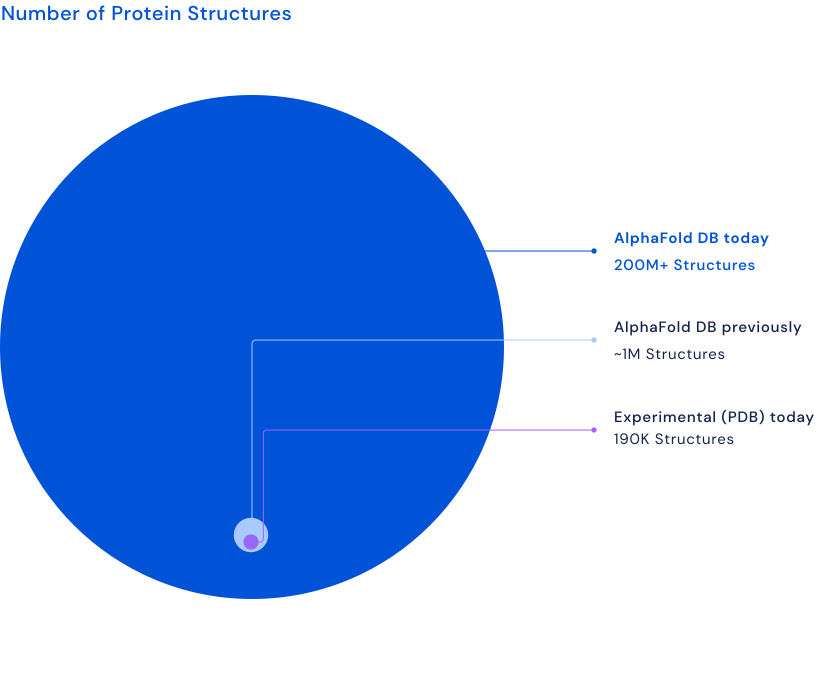
\includegraphics[width=0.8\linewidth]{files/alphafolddb-8b95e40845983ad2489efbbba10bacf9.pdf}
\caption[]{The most recent release includes predicted protein structures for plants, bacteria, animals, and other organisms, opening up many new opportunities for researchers to use AlphaFold to advance their work on important issues, including sustainability, food insecurity, and neglected diseases.
Note that PDB contains experimentally validated structures ({\textasciitilde}218K nowadays) and AlphaFold produces predicted structure models.
Credits: \cite{alphafolddb_2022}.}
\label{alphafolddb}
\end{figure}


\bigskip
\centerline{\rule{13cm}{0.4pt}}
\bigskip

\paragraph{Protein structure model quality}\label{chapter4_model_quality}

\begin{figure}[!htbp]
\centering
\includegraphics[width=0.7\linewidth]{files/7mfb-b7eb46c6c48f4dc3aab31ceb66e6eeea.png}
\caption[]{Heavy chain portion of the crystal structure of an antibody (PDB: 7MBF, in orange) superposed with the AlphaFold 2 prediction (in blue).
The overlay view shows how the folding of the two domains is largely predicted correctly, with some parts of the 3D protein structure that fit the PDB structure better than others.
Credits: \cite{blopig_2021}.}
\label{7mbf}
\end{figure}

Predictive models only have true value when they produce some measure of confidence, because without any idea of certainty about the predictions, it is hard to interpret results and draw conclusions.
To get an idea of how well predictions fit the reality, one needs to compare the model with the true situation.
Figure~\ref{7mbf} shows how this can be done by manual visual inspection of two super-imposed structures, the ``real'' (experimentally derived) one and a predicted one.
However, to quantitatively assess differences between models, some sort of numeric score is needed.
In this reader, we have seen one such comparative measure for 3D protein structure models in the CASP section: the Global Distance Test -- Total Score (Figure~\ref{casp}).
Another score you may encounter more often is the root mean squared error (RMSE), based on the difference in position of the~$\alpha$-carbons as input to calculate the score.
In principle, the smaller the RMSE of a model is, the better.
The QMEAN-DISCO score used by SWISS-MODEL is also used.
This score is an ensemble of various metrics that together provide insight into the quality of the model.

To assess the confidence in the model structure without a direct comparison to a known structure, one needs to assess the uncertainty in the position of the amino acid in the 3D coordinate system.
AlphaFold comes with its own local and global error predictions that the machine learning model calculates (see also AlphaFold~under~the~hood), and Figure~\ref{arf16}).
Where the local error focuses on individual positions of amino acids, the global error describes how confident the predictions are for various protein parts that can interact through residue-residue interactions.
The local error is also used to color-code the residues of the model in the 3D structure viewer.
In this way, it is easier to observe which parts of the structure model are more reliable than others.
You will study these two different error scores more during the practical assignment.

\begin{figure}[!htbp]
\centering
\includegraphics[width=0.7\linewidth]{files/arf16-c9eeddfe789bb86e7885fb020d6238b2.png}
\caption[]{Left: AlphaFold 3D protein structure model of Auxin Response Factor 16.
The amino acid residues are colored according to the local confidence score (see \href{https://alphafold.ebi.ac.uk/entry/A3B9A0\#help}{AlphaFold-PSD} and practical assignment for further explanation).
Right: the AlphaFold global error confidence score overview.
This view shows low errors (dark green) for two parts of the protein structure model, and higher errors for the remaining structure -- these also correspond to less confidence locally (see \href{https://alphafold.ebi.ac.uk/entry/A3B9A0\#help}{AlphaFold-PSD} and practical assignment for further explanation).
The structure model can be used to validate the protein's predicted function and can act as a starting point for further annotations, such as finding its biological interaction partners (i.e., other proteins, DNA, small molecules).
Credits: \href{https://creativecommons.org/licenses/by/4.0/}{CC BY 4.0} \cite{arf16_2022}.}
\label{arf16}
\end{figure}

As you may have started to realize when using databases, they can also contain erratic entries.
To investigate the quality of both known and predicted 3D protein structures, the Ramachandran plot can be used (chapter~1).
You will work with the Ramachandran plot during the practical assignments.
It is important to note here that some disordered proteins only come into orderly arrangement in the presence of their various protein partners; and other proteins never have ordered structures under any conditions, a property that may be essential to their function.
How to best model the behavior of such proteins is still an area of active research.

The above-described confidence measures are also useful in highlighting limitations of a predictive approach.
In the AlphaFold-related practical assignment, you will see some examples of this.
The main lesson is that you must treat a prediction as a prediction: it is a model of reality and may not accurately represent it.
Also, keep in mind that there are parts of the 3D protein structure that we can naturally be more confident about.
For example, secondary structure oftentimes supports the 3D protein structure, and parts of the protein that are naturally more disordered such as random loops are harder to predict correctly.
Such parts can typically represent parts of the protein structure that are more flexible in their biological environment and any prediction of (very) flexible parts should be considered as a snapshot of the protein structure.
If you study Figure~\ref{7mbf} in more detail, you will see this reflected in the superimposed image of the PDB (experimental) 3D structure and the AlphaFold structure model. In figure Figure~\ref{arf16} you can see the prediction model is more confident with the less flexible parts in the center of the protein and less confident with the flexible parts on the outer edges of the protein.


\bigskip
\centerline{\rule{13cm}{0.4pt}}
\bigskip

\paragraph{A protein structure model: and now?!}

Imagine you have generated a protein structure model, such as the one in Figure~\ref{7mbf}.
What can you do with it? As mentioned above, it can yield insights into its possible function and role in biochemistry.
In other words, you can start to form hypotheses that can be experimentally tested in the lab.
You can also start to make predictions of protein-protein interactions.
Since such interactions are typically driven by 3D structural elements (clefts, pockets, etc.), predicting such 3D structure elements from sequences will contribute to more confidently predicting protein-protein interactions.
Furthermore, you have seen how comparing protein sequences in multiple sequence alignments helps to gain insight into their relationships; by using 3D structure models as an input, a similar comparison could be done at the structural level.
As we are increasingly aware, sequences may deviate more than structural elements; thus, (multiple) structure alignments at the level of folds or subunits may give a different view on protein relationships.


\bigskip
\centerline{\rule{13cm}{0.4pt}}
\bigskip

\subsubsection{Foldseek}

A recent tool that allows to do structure-based alignments based on protein structure input in a reasonable timeframe is \href{https://search.foldseek.com/}{Foldseek} \cite{foldseek_2024}.
By designing a novel 3D-interactions (3Di) alphabet, the team behind Foldseek overcame the mounting task of doing structure-based comparisons at the very large scale that the availability of \textgreater 200 million structures, sparked by AlphaFold, requires.
For example, a traditional structure-based alignment tool would take {\textasciitilde}1 month to compare one structure to 100 million ones in the database.

% #% Add section about the 3Di alphabet and the use of substitution matrices in comparison to chapter 2 + a figure to visualise this.

During the practical assignments, you will explore how the combination of AlphaFold and Foldseek can be used to explore possible functions for a protein sequence of interest.


\bigskip
\centerline{\rule{13cm}{0.4pt}}
\bigskip

\subsubsection{Tertiary structure prediction outlook}

It can be expected that the AlphaFold model will continue to develop.
For example, the most recent addition in AlphaFold 3 is joint structure prediction of complexes including proteins, nucleic acids, small molecules, ions, and modified residues (Figure~\ref{alphafold3_prot_dna_ion}).

\begin{figure}[!htbp]
\centering
\includegraphics[width=0.7\linewidth]{files/alphafold3-prot-dna--0b1d2402b71eb07caf6702d78cec291c.png}
\caption[]{Example of a joint structure prediction of a \href{https://www.rcsb.org/structure/7RCE}{7RCE} protein interacting with a section of double helix DNA and two ions (Ca\textsuperscript{2}\textsuperscript{.} and Na\textsuperscript{.}) made with AlphaFold Server.
Credits: \cite{alphafold3_approach_2024}.}
\label{alphafold3_prot_dna_ion}
\end{figure}

This recent trend indicates a development in structure prediction from singular structure types to multiple structure types and a paradigm shift from sequence to structure based research.

Another topic of interest is modelling protein dynamics.
Many proteins can change shape and thereby function, for example depending on cellular conditions, but this is still very hard to model.
Finally, we are only starting to explore the role of post-translational modifications in generating many (structurally, functionally) different versions of each protein, so-called proteoforms.
Based on its current performance, it will be exciting to see where the field is ten years from now.
Akin to the mobile phone - smartphone development we have witnessed over the last decade, we may be surprised by its capabilities by then.

\begin{framed}
\textbf{Note 4.1}\\
Recently, the \href{https://openfold.io/}{OpenFold Consortium} has released their faithful but trainable PyTorch reproduction of DeepMind's AlphaFold 2. This is an open access machine-learning model that is publicly availble on their \href{https://github.com/aqlaboratory/openfold}{GitHub}.
OpenFold strives to deliver state-of-the-art AI-based protein modeling tools to researchers and commercial companies alike, who will be able to use, improve, and contribute to the development of the modeling tools themselves.
Developments like this improve the FAIRness (chapter~1) of the rapidly evolving field of tertiary structure prediction.
\end{framed}


\bigskip
\centerline{\rule{13cm}{0.4pt}}
\bigskip

\subsubsection{Closing remarks}

\begin{framed}
\textbf{Test your knowledge now!}\\
Have you read the above? Test yourself directly by answering the questions first and then revealing the answer by clicking on the question. Correct? Great! If not, you are encouraged to reread the part of the above section that deals with the questioned topic.
\end{framed}

\begin{framed}
\textbf{See Also}\\
Below, you will find several links with further information about protein structure prediction and AlphaFold.
Please note that these are not part of the exam material, which is covered above in this reader.
A number of these resources were used as an inspiration for the reader material.

Video introduction by the AlphaFold team:

\href{https://www.deepmind.com/blog/alphafold-a-solution-to-a-50-year-old-grand-challenge-in-biology}{Brief AlphaFold introduction by Deepmind}.

\href{https://www.deepmind.com/research/highlighted-research/alphafold/timeline-of-a-breakthrough}{History of AlphaFold}.

\href{https://blog.google/technology/ai/google-deepmind-isomorphic-alphafold-3-ai-model/}{AlphaFold most recent update}.

\href{https://www.nature.com/articles/s41586-021-03819-2}{AlphaFold 2 Nature publication}.

\cite{alphafold3_approach_2024}.

\href{https://www.blopig.com/blog/2021/07/alphafold-2-is-here-whats-behind-the-structure-prediction-miracle/}{A blogpost on AlphaFold 2}.

\href{https://alphafold.ebi.ac.uk/faq\#faq-5}{Good pointers on confidence in protein models}.

\href{https://www.nature.com/articles/s41587-023-01773-0}{Foldseek publication}.

\cite{deeptmhmm_2022}.

\href{https://elearning.vib.be/courses/alphafold/}{Inspiration and figures for this chapter} (\href{https://creativecommons.org/licenses/by/4.0/}{CC BY 4.0}). By Jasper Zuallaert (VIB-UGent), with the help of Alexander Botzki (VIB) and Kenneth Hoste (UGent).
\end{framed}

% PRACTICAL_SEPARATOR%


\bigskip
\centerline{\rule{13cm}{0.4pt}}
\bigskip

\subsection{Practical assignments}

This practical contains questions and exercises to help you process the study materials of Chapter 4.
You have 2 mornings to work your way through the exercises.
In a single session you should aim to get about halfway through this block, i.e., assignments I-III, but preferably being halfway with assignment IV.
These practical exercises offer you the best preparation for the project in Week 6 and the tools and their use are also part of the exam material.
Thus, make sure that you develop your practical skills now, in order to apply them during the project and to demonstrate your observation and interpretation skills during the exam.

\textbf{Note, the answers will be published after the practical!}

\begin{framed}
\textbf{\textbf{Project Preparation Exercise}}\\
This assignment is a project-like question: to remind you, the difference is that you will not be guided to the exact tools you need to use, but we rather expect you to use the knowledge and expertise from the reader and practical assignments to find the right tools.
In other words, this assignment is meant to let you explore the tools you have visited during the assignments I -- V (or alternative tools that you may have found) and come to relevant observations about the structure and function of the proteins under study.
After completing this assignment, you will be able to investigate known properties and predict likely properties of a protein based on its sequence and structure.

We continue our quest into members of the ARF gene family in \textit{Arabidopsis thaliana}.
You will remember that ARF5 (UniProt ID P93024) and IAA5 (UniProt ID P33078) are two well-studied \textit{A. thaliana} proteins that play a role in auxin-mediated regulation of gene expression.

As you will have realized by now, this chapter is all about structure and function!

\begin{itemize}
\item Shortly explore the 3D structures of both ARF5 and IAA5 -- how does structure support function? Which secondary structure elements are important? What drives the interaction between ARFs and IAAs? Which domains can you find? What can you learn about their functions?
\item Perform 2D structure prediction on both ARF5 and IAA5 and compare the results to the 3D structures.
\item Select one ARF or IAA in UniProt for which no experimental 3D structure is available in PDB. Follow the described biological discovery pipeline and use secondary and tertiary structure prediction to describe this sequence. What can you report?
\end{itemize}

Write short bullet point style notes for the three mentioned points below (please note that for the project, you will need to write short blocks of text rather than bullet points).
You may want to highlight some of your findings with screenshots from the tools that you visited -- use up to 6 Figures for this assignment.

\begin{enumerate}
\item \textbf{Materials \& Methods} What did you do? Which data, databases and tools did you use, and why did you choose these? What important settings did you select?
\item \textbf{Results} What did you find, what are the main results? Report the relevant data, numbers, tables/figures, and clearly describe your observations.
\item \textbf{Discussion \& Conclusion} Think about if the results you find make sense. Are they according to your expectation or do you see something surprising? What do the results mean, how can you interpret them? Do different tools agree or not? What can you conclude? Make sure to describe the expectations and assumptions underlying your interpretation.
\end{enumerate}

We encourage you to discuss your results with fellow students and the TAs and teacher.
Oftentimes, they may have found different but complementary information, and together you will be able to paint a more complete picture of the protein families.
\end{framed}

\subsection{Glossary}

\subsection{References}